\documentclass[11pt]{article}
\usepackage[a4paper,margin=1in]{geometry}
\usepackage{amsmath,amssymb,amsthm,mathtools}
\usepackage{booktabs}
\usepackage{array}
\usepackage{enumitem}
\usepackage{float}
\usepackage{graphicx}
\usepackage{hyperref}
\usepackage[nameinlink,capitalise]{cleveref}
\usepackage[numbers,sort&compress]{natbib}

\newtheorem{theorem}{Theorem}[section]
\newtheorem{proposition}[theorem]{Proposition}
\newtheorem{corollary}[theorem]{Corollary}
\newtheorem{remark}[theorem]{Remark}
\theoremstyle{definition}
\newtheorem{definition}[theorem]{Definition}
\newcommand{\norm}[1]{\left\lVert#1\right\rVert}
\newcolumntype{L}[1]{>{\raggedright\arraybackslash}p{#1}}

\title{Validated Folded-Gaussian Assembly and Exact Stochastic Repair\\
\large Algebraic Midpoint Rows, $8\sigma$ Truncation, Haar Compression, and a Perron-Exact Upstream Split}
\author{Liang Wang}
\date{July 2026}

\begin{document}
\maketitle

\begin{abstract}
RH-70 proved rigorous terminal Hardy bounds for the frozen matrices emitted by
the production pipeline, while RH-71 localized the finite-scale open frontier
to the upstream operator/source/observation triple.  This paper validates the
first part of that frontier: folded-Gaussian matrix and Haar block assembly.

Let $u_*$ be the unique root in $(1,2)$ of
$u^3-2u^2+2u-2=0$.  At positive midpoint nodes $x_i,y_j$, define
\[
 g_{ij}=
 \exp\!\left(-\frac{(y_j-(1-u_*x_i^2))^2}{2\sigma^2}\right)
 +
 \exp\!\left(-\frac{(-y_j-(1-u_*x_i^2))^2}{2\sigma^2}\right).
\]
The fully normalized row is $p_{ij}=g_{ij}/\sum_jg_{ij}$.  If $s_i$ is the
same row restricted to the production support and renormalized, then the
exact identity
\[
 \norm{p_i-s_i}_1
 =2\,\frac{\sum_{j\notin J_i}g_{ij}}{\sum_jg_{ij}}
\]
turns the truncation audit into one positive mass ratio.

For a frozen nonnegative binary64 row $f_i$, leave every entry except its
largest unchanged and set the largest entry equal to one minus the exact
dyadic sum of the others.  Whenever that replacement is positive, the
repaired row $\bar f_i$ is exactly stochastic,
\[
 \norm{\bar f_i-f_i}_1
 =\left|1-\sum_jf_{ij}\right|,
\]
and the constant vector is an exact Perron right vector.  Outward-rounded
absolute row and column sums $R,C$ then imply
\[
 \norm{P-\bar F}_2\le\sqrt{RC}.
\]
We also propagate this defect through exact and frozen Haar coarse/detail
embeddings by an explicit three-term product bound.

A 192-bit Arb audit covers
$\sigma=0.16,0.08,0.04,0.02,0.01$ and dimensions $32$ through $512$.
Every support-center floor is interval-stable.  The largest full-to-sparse
row defect is below $9.58\times10^{-17}$; the finest
$\norm{P-\bar F}_2$ upper is $1.495\times10^{-14}$; and every Haar
coarse/cross assembly defect is below $1.538\times10^{-14}$.  Exact row
repairs are below $3.87\times10^{-16}$ and every repaired pivot exceeds
$0.0775$.

Thus kernel evaluation, support selection, sparse renormalization, Haar
assembly, and the Perron right vector are green at the archived scales.  The
remaining finite-scale spectral gate is the stationary Perron left vector and
the parity Riesz pair.  This paper does not validate rank-two deflation,
prove small-noise uniformity, close Stage A1 or A4, construct a
Hilbert--Polya operator, derive a $T\log T$ law or prime-power trace formula,
or prove the Riemann Hypothesis.
\end{abstract}

\noindent\textbf{Keywords:} folded Gaussian kernel; interval arithmetic;
stochastic repair; Perron vector; Haar compression; validated assembly.

\medskip
\noindent\textbf{MSC 2020:} 47A10; 47B65; 60J20; 65G20; 65F35.

\section{Introduction}

The quadratic map
\[
 f_u(x)=1-ux^2
\]
at its first band-merging parameter supplies the deterministic geometry used
throughout the RH series \citep{WangKneading2026,WangBoundary2026}.  The noisy
positive-state transfer matrix is obtained by folding a Gaussian kernel,
truncating to a finite support, and normalizing every row.

RH-70 began only after that process and after spectral deflation: it embedded
the resulting binary64 operator, source, and observation arrays as exact
dyadic Arb/Acb inputs \citep{WangFrozen2026}.  RH-71 therefore identified
upstream inclusion as the next finite-scale gate \citep{WangReview2026}.

The upstream calculation contains two conceptually different tasks:

\begin{enumerate}[leftmargin=2.2em]
 \item evaluate and normalize the folded-Gaussian and Haar blocks;
 \item extract the stationary left factor and the parity Riesz pair.
\end{enumerate}

The first is positive scalar arithmetic; the second is a nonnormal spectral
problem.  This paper separates them.  Such separation avoids hiding a
spectral conditioning issue inside a large interval matrix constructor.

\subsection*{Contributions}

\begin{enumerate}[leftmargin=2.2em]
 \item We certify the algebraic parameter by a monotone polynomial interval.
 \item We derive an exact full-versus-support-renormalized row identity.
 \item We construct an exact dyadic stochastic repair of every frozen row.
 \item We turn entrywise interval differences into induced two-norm bounds.
 \item We propagate the matrix and $2^{-1/2}$ defects through coarse/detail
       Haar products.
 \item We execute the entire assembly audit at the five RH-70 scales.
\end{enumerate}

\section{The algebraic folded midpoint matrix}
\label{sec:matrix}

Let
\[
 q(u)=u^3-2u^2+2u-2.
\]
The parameter $u_*$ is the first band-merging root.

\begin{proposition}[Certified algebraic parameter]
\label{prop:root}
The interval
\[
 \begin{split}
 I_*={}&[1.5436890126920763615708559718017479865252032976510\\
 &\hspace{3em}{}\pm2.61\times10^{-50}]
 \end{split}
\]
contains exactly one root of $q$.
\end{proposition}

\begin{proof}
Outward-rounded evaluation gives a negative upper endpoint for $q$ at the
left endpoint of $I_*$ and a positive lower endpoint at the right endpoint.
Moreover,
\[
 q'(I_*)=3I_*^2-4I_*+2
 \subset[2.9741712529504070\ldots\pm3.40\times10^{-49}],
\]
whose lower endpoint is positive.  The intermediate value theorem and strict
monotonicity give existence and uniqueness.
\end{proof}

For dimension $n$, put
\[
 x_i=y_i=\frac{i+1/2}{n},
 \qquad 0\le i<n,
\]
and $\mu_i=1-u_*x_i^2$.  The unnormalized folded weights are
\begin{equation}
 g_{ij}=
 e^{-(y_j-\mu_i)^2/(2\sigma^2)}
 +e^{-(-y_j-\mu_i)^2/(2\sigma^2)}.
 \label{eq:weight}
\end{equation}
The common Gaussian prefactor cancels under row normalization.

Define the full midpoint matrix
\begin{equation}
 P_{ij}=\frac{g_{ij}}{Z_i},
 \qquad
 Z_i=\sum_{j=0}^{n-1}g_{ij}.
 \label{eq:full}
\end{equation}
Thus $P\mathbf1=\mathbf1$ exactly.

\section{Exact support-truncation identity}
\label{sec:truncation}

Let $J_i$ be the support used by the production sparse row.  Put
\[
 Z_{i,J}=\sum_{j\in J_i}g_{ij},
 \qquad
 Z_{i,\mathrm{out}}=Z_i-Z_{i,J},
\]
and
\[
 S_{ij}=
 \begin{cases}
  g_{ij}/Z_{i,J},&j\in J_i,\\
  0,&j\notin J_i.
 \end{cases}
\]

\begin{theorem}[Full/sparse row identity]
\label{thm:truncation}
For every row with positive weights,
\begin{equation}
 \norm{P_i-S_i}_1
 =2\frac{Z_{i,\mathrm{out}}}{Z_i}.
 \label{eq:l1}
\end{equation}
\end{theorem}

\begin{proof}
On the retained support, $Z_{i,J}\le Z_i$, so
\[
 \sum_{j\in J_i}
 \left(\frac{g_{ij}}{Z_{i,J}}-\frac{g_{ij}}{Z_i}\right)
 =1-\frac{Z_{i,J}}{Z_i}
 =\frac{Z_{i,\mathrm{out}}}{Z_i}.
\]
The omitted coordinates contribute the same quantity:
\[
 \sum_{j\notin J_i}\frac{g_{ij}}{Z_i}
 =\frac{Z_{i,\mathrm{out}}}{Z_i}.
\]
Adding proves \eqref{eq:l1}.
\end{proof}

The production support center is
\[
 c_i=\left\lfloor n|\mu_i|-\frac12\right\rfloor
\]
with half-width $\lceil8\sigma n\rceil+2$.  The interval run verifies that
the lower and upper endpoints give the same floor for every row.  Therefore
support selection itself is stable under the certified algebraic parameter
interval.

\section{Exact stochastic repair}
\label{sec:repair}

Binary64 row normalization generally leaves a tiny exact-dyadic row-sum
defect.  Treating the rounded row as exact does not make that defect vanish
\citep{Higham2002}.

Let $f=(f_0,\ldots,f_{n-1})$ be a nonnegative dyadic row and choose an index
$k$ with maximal entry.  Define
\begin{equation}
 \bar f_j=f_j\quad(j\ne k),
 \qquad
 \bar f_k=1-\sum_{j\ne k}f_j.
 \label{eq:repair}
\end{equation}

\begin{theorem}[Exact dyadic stochastic repair]
\label{thm:repair}
If the replacement in \eqref{eq:repair} is positive, then:
\begin{enumerate}[label=(\roman*),leftmargin=2.2em]
 \item every $\bar f_j$ is a nonnegative dyadic rational and
       $\sum_j\bar f_j=1$ exactly;
 \item
 \begin{equation}
  \norm{\bar f-f}_1
  =\left|1-\sum_jf_j\right|;
  \label{eq:repair-distance}
 \end{equation}
 \item for the rowwise repaired matrix $\bar F$,
       $\bar F\mathbf1=\mathbf1$ exactly and
 \begin{equation}
  \norm{\bar F-F}_\infty
  =\max_i\left|1-\sum_jF_{ij}\right|.
  \label{eq:repair-matrix}
 \end{equation}
\end{enumerate}
\end{theorem}

\begin{proof}
Finite sums and differences of dyadic rationals are dyadic.  The definition
forces exact row sum one.  Only coordinate $k$ changes, by
$1-\sum_jf_j$, giving \eqref{eq:repair-distance}.  Taking the maximum row
$\ell^1$ norm gives \eqref{eq:repair-matrix}; exact stochasticity gives the
Perron right-vector statement.
\end{proof}

The repair need not be stored as binary64: it is an exact dyadic rational
accepted directly by Arb.  Its floating display is only a convenience.

\section{From entry balls to matrix and Haar bounds}
\label{sec:norms}

Let $D=P-\bar F$.  Suppose outward-rounded accumulation gives
\[
 R\ge\max_i\sum_j|D_{ij}|,
 \qquad
 C\ge\max_j\sum_i|D_{ij}|.
\]

\begin{proposition}[Induced two-norm enclosure]
\label{prop:two}
\begin{equation}
 \norm D_2\le\sqrt{\norm D_1\norm D_\infty}\le\sqrt{CR}.
 \label{eq:two}
\end{equation}
\end{proposition}

\begin{proof}
This is the standard induced-norm inequality, with the two induced norms
bounded by the certified absolute column and row sums.
\end{proof}

Let $E,D_H\in\mathbb R^{n\times n/2}$ be the exact Haar coarse and detail
embeddings with entries $\pm2^{-1/2}$, and let $E_0,D_{H,0}$ use the frozen
binary64 constant.  Their defects satisfy
\[
 \delta_H=\norm{E-E_0}_2=\norm{D_H-D_{H,0}}_2
 =\sqrt2\left|2^{-1/2}-\operatorname{fl}(2^{-1/2})\right|.
\]

\begin{theorem}[Haar compressed assembly bound]
\label{thm:haar}
Let $X,Y$ independently denote either the exact coarse or detail embedding,
and $X_0,Y_0$ the matching frozen embeddings.  Then
\begin{equation}
 \norm{X^*PY-X_0^*\bar F Y_0}_2
 \le
 \norm{P-\bar F}_2
 \delta_H\norm{\bar F}_2
 \norm{X_0}_2\norm{\bar F}_2\delta_H.
 \label{eq:haar}
\end{equation}
The same upper therefore applies to the coarse matrix and both coarse/detail
cross blocks.
\end{theorem}

\begin{proof}
Insert and subtract $X^*\bar F Y$ and $X_0^*\bar F Y$:
\[
 X^*PY-X_0^*\bar F Y_0
 =X^*(P-\bar F)Y
 +(X-X_0)^*\bar F Y
 +X_0^*\bar F(Y-Y_0).
\]
Use $\norm X_2=\norm Y_2=1$ and submultiplicativity.
\end{proof}

\section{Five-scale interval audit}
\label{sec:audit}

The implementation uses 192-bit Arb arithmetic \citep{Johansson2017}.  The
algebraic parameter is an interval; midpoint nodes and $\sigma$ are exact
rationals; every exponential, row total, division, absolute difference, row
sum, and column sum is outward rounded.  Frozen binary64 entries are embedded
as their exact dyadic ratios.

\begin{table}[H]
\centering
\small
\caption{Validated assembly bounds.  The compressed column is the common
two-norm upper for coarse and cross-block assembly against the repaired
pipeline.}
\label{tab:audit}
\begin{tabular}{rrrrrr}
\toprule
$\sigma$ & $n$ & max truncation $L^1$ &
$\norm{P-\bar F}_2$ & compressed defect & max repair\\
\midrule
0.16 &  32 & $0$                    & $6.377\times10^{-16}$ & $8.560\times10^{-16}$ & $1.374\times10^{-16}$\\
0.08 &  64 & $9.088\times10^{-17}$ & $1.295\times10^{-15}$ & $1.555\times10^{-15}$ & $2.528\times10^{-16}$\\
0.04 & 128 & $8.510\times10^{-17}$ & $2.459\times10^{-15}$ & $2.767\times10^{-15}$ & $3.406\times10^{-16}$\\
0.02 & 256 & $9.520\times10^{-17}$ & $6.175\times10^{-15}$ & $6.541\times10^{-15}$ & $3.862\times10^{-16}$\\
0.01 & 512 & $9.577\times10^{-17}$ & $1.495\times10^{-14}$ & $1.538\times10^{-14}$ & $3.776\times10^{-16}$\\
\bottomrule
\end{tabular}
\end{table}

The exact Haar embedding defect is
\[
 \delta_H\le8.86511592918\times10^{-17}.
\]
The smallest repaired pivot lower endpoint over all rows and scales is above
$0.0775500$, so positivity is separated from zero by fourteen orders of
magnitude more than the repair.

The minimum support-center distance from an integer threshold is
$9.85\times10^{-4}$ at the finest scale.  Thus the archived support pattern
is not close to changing under the algebraic parameter enclosure.

\begin{figure}[H]
\centering
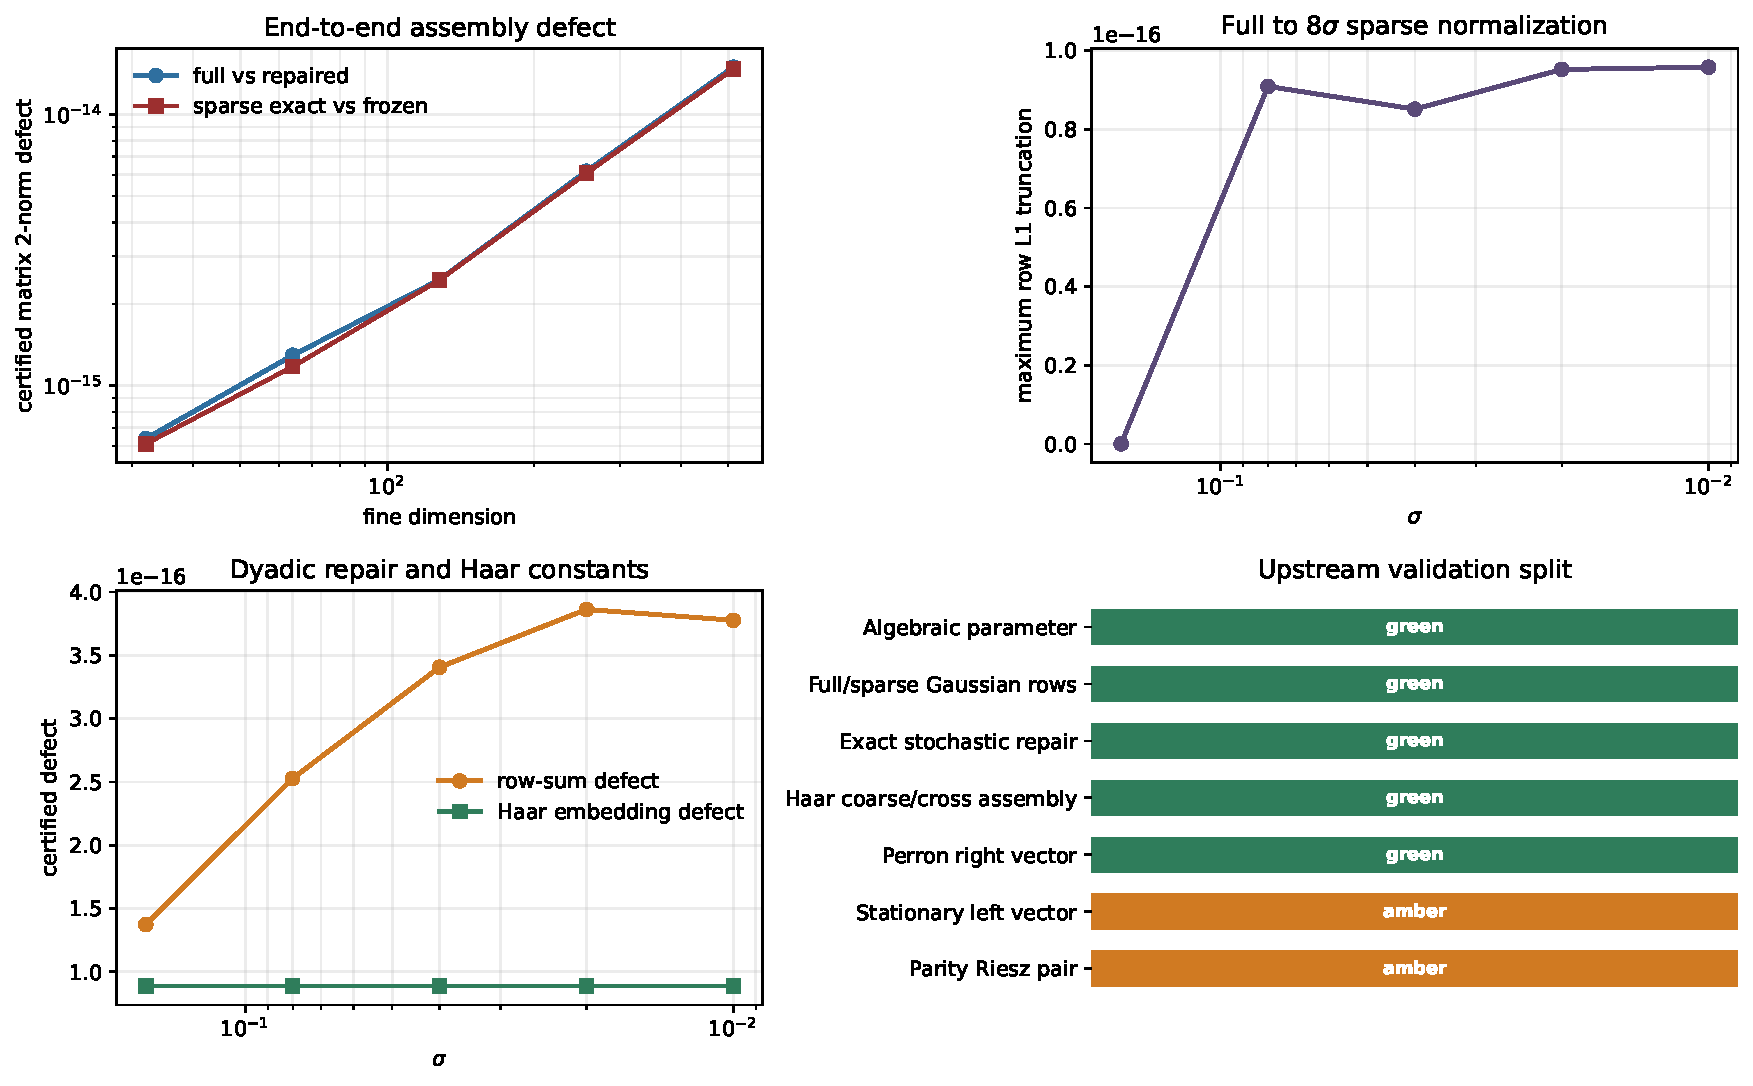
\includegraphics[width=0.98\textwidth]{figures/validated_folded_gaussian_assembly.pdf}
\caption{Full/frozen assembly defects, $8\sigma$ truncation, exact dyadic
repair and Haar constants, and the resulting upstream validation split.}
\label{fig:audit}
\end{figure}

\section{Route consequence}
\label{sec:route}

The finite-scale upstream graph may now be refined:
\[
\boxed{
\begin{array}{c}
\text{algebraic full midpoint rows}\\
\downarrow\\
\text{sparse support and exact stochastic repair}\\
\downarrow\\
\text{Haar coarse/detail blocks}
\end{array}}
\quad\text{green},
\]
while
\[
\boxed{
\text{stationary left factor}
\;+\;
\text{parity Riesz pair}
\;+\;
\text{rank-two subtraction}}
\quad\text{amber}.
\]

The exact stochastic repair is especially useful.  It removes the need to
validate the Perron \emph{right} vector numerically: $\mathbf1$ is exact.
RH-73 can therefore focus on a stationary left solve and one parity
left/right pair, followed by biorthogonal normalization.

\section{Boundary and nonclaims}

The target here is the fully normalized midpoint matrix, not the continuum
operator or exact cell-averaged Ulam matrix.  The earlier strong--weak theory
provides the analytic midpoint/cutoff route \citep{WangStrongWeak2026}; this
paper does not re-prove it.

Five finite scales do not prove a uniform small-noise assembly theorem,
although the displayed errors remain at floating-roundoff scale.  More
importantly, this paper does not validate the stationary left vector, parity
eigenvalue/eigenvectors, rank-two projector, deflated bulk operator, or the
complete source/observation triple.  Hence finite-scale end-to-end Stage A1
is not yet closed.

No Stage A4 identification, pole-renormalized determinant, canonical
scattering object, self-adjoint Hilbert--Polya generator, $T\log T$ counting
law, prime-power trace formula, completed-zeta identity, or Riemann
Hypothesis conclusion is claimed.

\section{Conclusion}

The folded-Gaussian upstream gate separates cleanly.  Positive scalar
assembly---including the algebraic parameter, full midpoint weights,
$8\sigma$ support, row normalization, stochastic repair, and Haar
compression---is rigorously stable at all five production scales.  The
largest complete matrix defect is $1.5\times10^{-14}$.

The next wall is genuinely spectral rather than numerical assembly:
validate the stationary left vector and parity Riesz pair, then propagate
their rank-two subtraction through the source and observation blocks.

\bibliographystyle{plainnat}
\bibliography{references}

\end{document}
